\chapter{根因分析} % Introduction chapter suppressed from the table of contents

某美国学者到日本做培训,晚上好客的日本人请他去夜总会,他发现年轻的女服务员腰上都有一个英文Q字牌子,他很好奇,问原因。原来这家夜总会刚完成几个月的过程改进,得到日本政府奖励金,所以都挂上这个Q牌(Q代表Quality质量)。

以下让我们看看夜总会如何做过程改进。

%\href{文件:club11.jpg}{400px}

%\includegraphics[width=10cm]{club11.jpg}

 %日式夜总会的过程改进

\hypertarget{esquire-qcux5708}{%
\subsection{Esquire QC圈}\label{esquire-qcux5708}}

QC圈成立于1984年12月,由Sakae领导,加上下面的女服务员。

当时,Sakae
43岁,有七个月的经验。除了她,圈内7女服务员的年龄从19岁到23岁不等。

\hypertarget{ux7528ux4e8cux516bux539fux5219-paretoux56fe-ux8bc6ux522bux4e3bux8981ux6e90ux5934}{%
\subsection{用二八原则 (Pareto图)
识别主要源头}\label{ux7528ux4e8cux516bux539fux5219-paretoux56fe-ux8bc6ux522bux4e3bux8981ux6e90ux5934}}

\begin{itemize}
\tightlist
\item
  发现 清酒 (sake) 与 啤酒 (beer) 是最大的源头
\end{itemize}

%\href{文件:club55.png}{600px}

\includegraphics[width=10cm]{club55.png}

%\href{文件:club6.png}{600px}

\includegraphics[width=10cm]{club6.png}

%\href{文件:club7.png}{600px}

\includegraphics[width=10cm]{club7.png}

%\href{文件:club8.png}{600px}

\includegraphics[width=10cm]{club8.png}

%\href{文件:club9.png}{600px}

\includegraphics[width=10cm]{club9.png}

从10月份到 2月份,啤酒和清酒的平均每月损失是 4万9千日元。

\hypertarget{ux5efaux7acbux76eeux6807}{%
\subsection{建立目标}\label{ux5efaux7acbux76eeux6807}}

目标:把损失减半 (少50\%):
从目前每月平均损失89瓶啤酒和17升清酒,降到(不超过)44瓶啤酒和8升清酒。

\hypertarget{ux6839ux56e0ux5206ux6790-root-cause-analysis-ux9c7cux9aa8ux56feux5206ux6790}{%
\subsection{根因分析 Root Cause analysis ( 鱼骨图分析
)}\label{ux6839ux56e0ux5206ux6790-root-cause-analysis-ux9c7cux9aa8ux56feux5206ux6790}}

\begin{itemize}
\tightlist
\item
  大家头脑风暴,讨论分析啤酒和清酒损失的主要原因。
\item
  根据服务员、工作流程、其他等三个主线分析。
\end{itemize}

这三组构成因果图的三个主要分支。

%\href{文件:club111.png}{600px}

\includegraphics[width=10cm]{club111.png}

\textbf{鱼骨图每个分支的主要内容如下:}

%\href{文件:club12.1.jpg}{600px}

\includegraphics[width=10cm]{club121.jpg}

%\href{文件:club13.1.jpg}{600px}

\includegraphics[width=10cm]{club131.jpg}

%\href{文件:club14.1.jpg}{600px}

\includegraphics[width=10cm]{club141.jpg}

%\href{文件:club15.1.jpg}{600px}

\includegraphics[width=10cm]{club151.jpg}

基于上面的鱼骨图分析,大家讨论并想到了以下主要理由/原因:

\begin{itemize}
\tightlist
\item
  没有具体的固定位置放置票据
\end{itemize}

\begin{itemize}
\tightlist
\item
  依赖别人
\end{itemize}

\begin{itemize}
\tightlist
\item
  处理热清酒器不当
\end{itemize}

\begin{itemize}
\tightlist
\item
  价格计算有误
\end{itemize}

\begin{itemize}
\tightlist
\item
  分工有误 / 没有分配好工作
\end{itemize}

\begin{itemize}
\tightlist
\item
  准备不足
\end{itemize}

\begin{itemize}
\tightlist
\item
  对客户桌结算(喝了多少并收拾空酒瓶)频率不足。
\end{itemize}

\framebox{%
\begin{minipage}[t]{0.97\columnwidth}\raggedright
注意:
以上每一项都是问题的根本原因,很多人误以为针对问题本身,找改正措施便算根因分析。5
Why 方法可以帮助正确找到根因,详见附件``5 Why 例子``。\strut
\end{minipage}}

\hypertarget{ux6539ux8fdbux63aaux65bd}{%
\subsection{改进措施}\label{ux6539ux8fdbux63aaux65bd}}

\begin{itemize}
\tightlist
\item
  要确保留票据在桌子上,不带走
\end{itemize}

(在繁忙时段,在纸上标记消费了多少矿泉水,啤酒和日本清酒,贴在总单的后面,利于计算总账

\begin{itemize}
\tightlist
\item
  制定规程来分配各个区域的工作。每个小时每个区域负责人必须检查一次所有范围内的票据。
\end{itemize}

\begin{itemize}
\tightlist
\item
  送热毛巾的那位服务员负责记录新加入的客人
\end{itemize}

\begin{itemize}
\tightlist
\item
  谁接单谁负责记账,如果她要求其他人来协助记录,必须确保沟通好,检查是否已经做好记录。
\end{itemize}

\begin{itemize}
\tightlist
\item
  管理者必须对新成员提供培训,如新员工小组学习。
\end{itemize}

\begin{itemize}
\tightlist
\item
  以区域分桌,使大家清楚谁负责哪桌。
\end{itemize}

\hypertarget{ux6539ux8fdbux6548ux679c}{%
\subsection{改进效果}\label{ux6539ux8fdbux6548ux679c}}

%\href{文件:club19.png}{600px}

\includegraphics[width=10cm]{club19.png}

%\href{文件:club20.png}{600px}

\includegraphics[width=10cm]{club20.png}

%\href{文件:club21.png}{600px}

\includegraphics[width=10cm]{club21.png}

%\href{文件:club22.png}{600px}

\includegraphics[width=10cm]{club22.png}

以日元计算,啤酒和清酒的损失从每月平均4万9千日元减少到5687日元,减少了43,401日元,即88\%。这一降幅远超过最初设定的50\%的目标。

\hypertarget{a3ux62a5ux544a}{%
\subsection{A3报告}\label{a3ux62a5ux544a}}

很多给管理层的报告都非常厚, 信息太多导致管理者难以消化。
所以丰田要求所有管理报告都必须精简到一张A3纸。

照片中服务员手上的就是A3报告 -
包含了根因分析的重点。例如,你可以看见其中有鱼骨图。

\hypertarget{ux6280ux672fux603bux76d1ux7ecfux9a8cux4e4bux8c08}{%
\subsection{技术总监经验之谈}\label{ux6280ux672fux603bux76d1ux7ecfux9a8cux4e4bux8c08}}

\framebox{%
\begin{minipage}[t]{0.97\columnwidth}\raggedright
总监之前一直在日本带领开发团队,十年前回大陆。最近为他们做过程差距分析,我汇报他们根因分析的不足后,总监开车送我去机场时分享他的日本经历:\strut
\end{minipage}}

你说我们团队没有找出真正根因,我非常赞同。日本在根因分析做得特别好。我之前在日本工作,带领小组做开发,当时我们团队共5人,有2位来自大陆,其他是本地人,有一次,因为我们开发计算公积金出错,QA一直追问问题的原因。当时我还没有找出根因的概念,不明白QA的意图,以为只是问责,希望找个人背锅。其实他们确实是希望找出问题的源头,避免同类问题再发生。当主管追问原因,要求我发问题报告。我的报告只说了一些开发问题,人员经验不足等。主管一直追问为什么。``如果你说培训经验不足,你有什么培训相关的安排来避免?''我回答不上来。最后发现,原来是日本计算方法和大陆不同,他们不四舍五入,导致我们两位大陆开发人员的计算便和本地的不同。
很多大陆工程师没有根因分析概念,认为质量依靠个人保证 -
``我负责,有问题我承担''。日本人不是这个思路,他们希望挖掘到问题的根本原因,并避免。后面我回国发展,开始时兼职做咨询工作,帮一位老朋友看看某软件开发公司团队的问题,发现很多大陆团队对质量方面的要求远远不如日本,很不习惯。

\hypertarget{ux603bux7ed3}{%
\subsection{总结}\label{ux603bux7ed3}}

从以上案例可以了解根因分析的主因元素:\\
1.利用图识别引起大部分问题的最主要几个因素(因资源有限,必须有针对性)\\
2.分析背后的主要原因\\
3.对应改进措施\\
4.判断改进效果\\
5.总结成根因分析报告\\
因为过程改进要花费公司额外的资源投入, 必须有针对性管理层才会支持,
所以应利用二八原则识别哪几个主要因素的影响最大。
有些人以为只需要对某个维度做分析, 没有从多个维度分析。

例如,某纸制产品工厂会计数据显示
八成的产品问题相关成本都归属于5类,例如:质量不合格,赔偿,售后现场服务等(共有20类)
针对5类中最大的一类:质量不合格,
发现里面八成的成本都由于六个产品引起(共有50个产品)
针对这六个产品把成本按缺陷种类细分,发现B产品断裂缺陷的成本最高,
我们就应该针对这一问题研究如何改善。

%\href{文件:Ar2_缺陷类型造成的损失.jpg}{文件:Ar2 缺陷类型造成的损失.jpg}

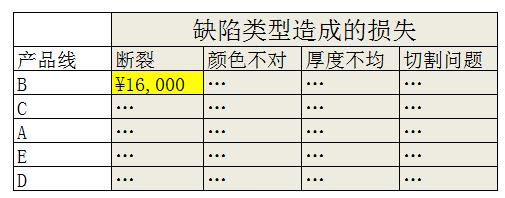
\includegraphics[width=10cm]{Ar2_缺陷类型造成的损失.jpg}

有时候找根因不一定靠头脑风暴或鱼骨图,如果细分到过程里那些步骤出问题,更有针对性。例如深圳某软件开发公司,每2周定期发版。如果有出现赶不上,不能在预定的发版时间发布软件,项目经理和项目组会非常注重,做复盘,一起分析过程出了那些问题导致不能按时发版。他们会按整个流程,每一步分析,但分析以定性头脑风暴为主。如果在分析过程中,对风险的发生概率、影响度和预先检测难易度都要打分,就可以量化分析,称为
故障模式与影响分析,详见附件``FMEA实例''。

\hypertarget{ux9644ux4ef6}{%
\section{附件}\label{ux9644ux4ef6}}

\hypertarget{why-ux4f8bux5b50}{%
\subsection{5 Why 例子}\label{why-ux4f8bux5b50}}

网上搜索``大野耐一 5 Why``应可找到以下例子:

\begin{description}
\tightlist
\item[]
(大野先生是丰田汽车总工程师,从50年代始一直主导丰田的质量改善。)
\end{description}

%\href{文件:5whyScreenshot_2022-12-03_092224.jpg}{500px}

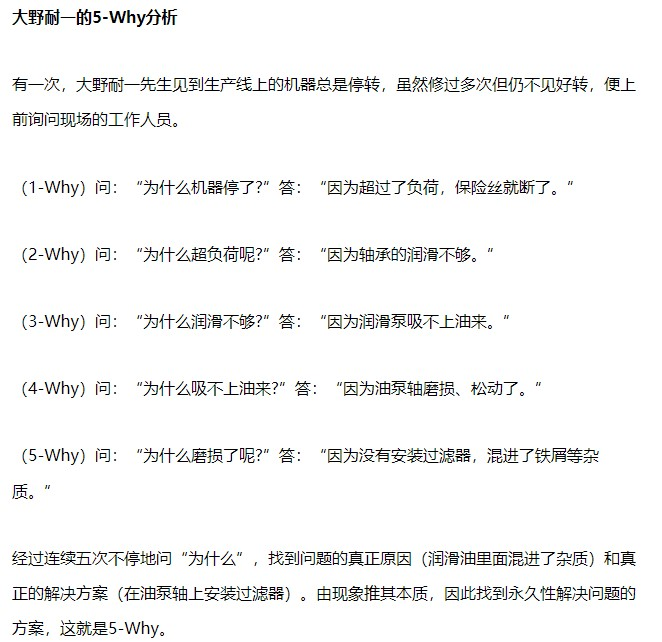
\includegraphics[width=10cm]{5whyScreenshot20221203092224.jpg}

\hypertarget{fmea-ux5b9eux4f8b}{%
\subsection{FMEA 实例}\label{fmea-ux5b9eux4f8b}}

\begin{description}
\tightlist
\item[]
(FMEA: Failure Mode Effects Analysis)
\end{description}

大家都可能试过未管理好时间,导致迟到。以坐飞机为例,从离开酒店到登上飞机过程中很可能有不少风险导致最后没搭上。\\
你出发的时候,可能用不同的交通方式:出租车、机场大巴等。如果你不能在起飞前45分钟到达机场办理登机牌,你便搭不上。但是你拿了登机牌也有可能最后搭不上,因为飞机都严格执行起飞前15分钟关舱门,所以你拿了登机牌也要在起飞前15分钟到达,才能顺利乘机。

Fig 1 登机过程

%\url{文件:风险与机会1.png}

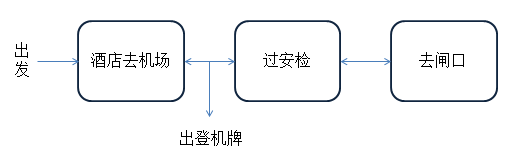
\includegraphics[width=10cm]{风险与机会1.png}

要赶上飞机其实是个过程,中间有很多环节会导致最后失败,所以我们可以用
FMEA 过程分析,来看如何控制减少失败的概率。

Fig 2 FMEA 例子

%\href{文件:风险与机会2_FMEA.png}{文件:风险与机会2 FMEA.png}

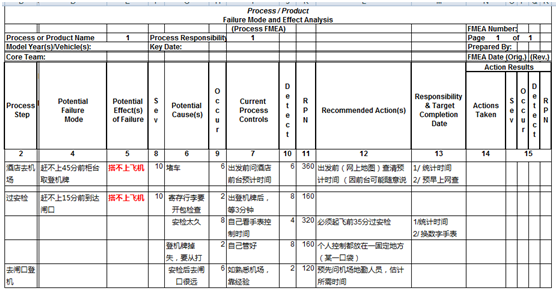
\includegraphics[width=10cm]{风险与机会2_FMEA.png}

Fig 3 打分参考

%\href{文件:风险与机会3_打分参考_1.png}{文件:风险与机会3 打分参考 1.png}

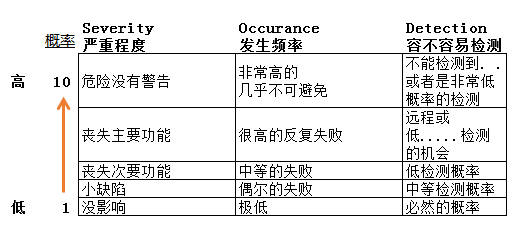
\includegraphics[width=10cm]{风险与机会3_打分参考_1.png}

以第一个失效为例:如发生便坐不上飞机,所以严重性是最高10。发生的概率还是比较高6。是否容易预防,预警,因不熟悉当地情况,加上我主要靠问酒店前台,有时候她也不清楚,所以我定6。RPN
= 10x6x6=360。

从以上登机的例子,可以看出FMEA是以整个过程来管理风险,比如在出发前,就要查询一下各个交通工具要花费的时间,比如你发现在南京,从酒店坐地铁要转车,要花1个小时以上,如果时间太紧就来不及,宁可多花钱打车,才能控制风险。
当你拿了登机牌,还是要经过安检,还要从安检走过登机口。有时候机场很大,到达登机口也要花很长时间,就要先问好路径,提前计算好时间,才不会误点。\\
过了安检到登机口要10分钟以上,就要在起飞前的35分钟完成通过安检,才来得及。这些都可以通过FMEA的形式把整个坐飞机的过程识别出来,找各个阶段会出现的问题,就知道如何控制。

以这坐飞机的风险为例,我自己是不仅一次有赶不上飞机,很多原因,但回顾一下都是习惯没改过来问题。我应依据以往差点赶不上的经验,回顾一下,确保每一个过程都控制住,就不会后面再次出问题
,这个和企业做风险管理概念一样。\\
有度量才有管理。人和公司一样,很多做的事情好像是自己主动去想,其实很多都是潜意识习惯,如果你没有定一些量化的控制手段,就不会提高这方面风险意识,还是会搭不上飞机。我先回顾以往几次搭飞机的情况,并把每次到达机场的时间和到达闸口的时间写下(详见下面
Fig 4 )\\
Fig 4 上面是机场柜台关闭(45分钟)前到达时间,下面是关闸口前到达时间
(分钟)( X 代表赶不上飞机)

%\url{文件:风险与机会4.png}

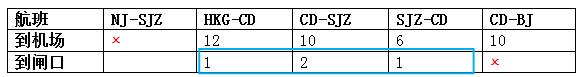
\includegraphics[width=10cm]{风险与机会4.png}

我发现最近一次赶不上飞机,之前已发生过两次刚刚赶到闸口 !\\
如果我有把经验教训记下来,下次做好时间管理,就会避免后面的延误:有了数据,我们便可以更有效在回顾时做好根因分析
(CAR)。\\
以这登记延误风险为例,可以使用FMEA分析每一失效点,例如过安检(因没有预留足够时间)与从安检到闸口太长时间等的发生概率都很高
(前者8, 后者 6)\\
为了避免问题再发生,就要定一些具体的计划,最终希望把误点减到零。\\
在登机这个环节,可利用什么有效方法/工具,帮助改善?

-
每次出发去机场前都查询各种交通方式的时间与风险(概率),预留足够时间,降低失效发生的概率\\
- 拿了登记牌后,都计划好必须起飞前35分通过安检,45分前开始安检

在多次没登上飞机后,我发现平常的手表没有正负5分钟的概念,但是如果用电子手表,对时间的感觉可以准确到了正负1分钟,就能够更好把控时间。

Fig 5 平常用于培训 / 评估计时的电子钟

%\href{文件:风险与机会5_闹钟.png}{文件:风险与机会5 闹钟.png}

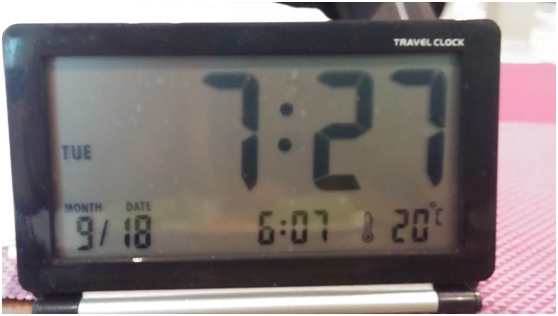
\includegraphics[width=10cm]{风险与机会5_闹钟.png}

经过这次误机,我就买了个电子手表,取代传统针式手表,希望对日后不迟到有帮助。

\textbf{效果}: 这故事发生在2019.9
,后面我按这些计划,一直都没有再出现赶不上飞机 -
我每次都提醒自己必须起飞前60 - 90分钟到机场,30 -
45分钟前到闸口。分析的目的是提高个人风险意识,避免问题发生。

团队了解了根本原因分析的原理与方法不代表能做好回顾分析,
例如,学生在培训里利用模拟数据,用鱼骨图和帕累托图做完互动练习,如他们只用这些技巧,难以做好回顾,下章继续分享敏捷回顾要注意的重点。



